\documentclass[11pt,letterpaper]{report}
\usepackage[latin1]{inputenc}
\usepackage[a4paper,margin=1in]{geometry} % set document margins
\usepackage{parskip}  % removes auto-indent and changes newline behavior
\usepackage{amsmath}
\usepackage{amsfonts}
\usepackage{amssymb}
\usepackage{subfig}
\usepackage{graphicx}
\usepackage{enumitem} % for enumerations
\usepackage{hyperref} % for hyperlinks
\usepackage{color}
\usepackage[]{algorithm2e}
%\graphicspath{ {/andykeene/Desktop/}}
\graphicspath{{./images/}{IR}}
\usepackage{fancyhdr}
\pagestyle{fancy}
\fancyhead{}
\lhead{CS350}
\chead{Empiricism and Asymptotic Promises}
\rhead{Keene}
\author{Andy Keene}
\title{Assignment X\\Algorithms and Complexity\\ Winter 2017}
\date{}
%	\maketitle
\hypersetup {
  colorlinks=true,
  urlcolor=blue
}
\begin{document}


\section*{Overview}
The relational ordering of data has remained a fundamental pursuit in many domains of computer science. Not only is this ordering intrinsically tied to many problems, such the creation and searching of data structures, but it also serves as a method of reduction from more complicated problems to feasibly solvable instances of another. Although many solutions to this problem have been proposed over the years only a few of these solutions have been granted membership into the exclusive class of efficient sorting algorithms. The two most preeminent of these solutions are arguably mergesort and quicksort. This paper is concerned with the comparison of empirical data to the asymptotic promises of each algorithms implementation. These two algorithms were chosen not only to justify their popularity, but also to contrast the varying approaches to constructing an efficient sorting algorithm and the tradeoffs that must be made in order to achieve this goal; thus illustrating algorithmic limitations.

\subsection*{Mergesort}			%Merge sort
Mergesort approaches the sorting problem by employing the popular and quite effective technique of divide and conquer. Given an array $A[0...n-1]$ of length $n$, merge sort continually divides the array in half until $n$ subarrays of length one exist. The beauty of this, known as the base case, is the ensured condition in which all arrays are sorted in some relational order - since any sequence of one is itself sorted. 

Next, merge sort takes each pair of adjacent subarrays $a$ and $b$, and \emph{merges} them into a new array $c$ where $|c|=|a+b|$. Because each subarray is already in sorted order, such that $a_1 \leq a_2 \leq ... \leq a_i$ and $b_1 \leq b_2 \leq ... \leq b_j$, merge sort must only insert the smallest of $a_1$ and $b_1$ as $c_1$. Continuing by inserting the smallest of the two remaining left-most elements between $a$ and $b$, it is clear each subsequently inserted element is larger than or equal to the last; yielding the array $c$ in the same relational sorted order as $a$ and $b$ (i.e. $c_1 \leq c_2 \leq ... \leq c_{i+j}$). If one array is emptied before the other, mergesort no longer compares but instead inserts the remaining elements from the non-empty array, either $a$ or $b$, into $c$.  Finally, the \emph{merging} ends with copying $c$ back into the original array $a$. The following diagram helps to illustrate this process: 

-- Picture Needed --

So the entire algorithms process may be thought of as obtaining two sorted subarrays via itself, then \emph{merging} the subarrays using the the process outlined above. Pseudo-code describing the recursive implementation is given as:

\begin{algorithm}[H]
\textbf{Mergesort} $(A[b....t], b, t)$ \\
 \eIf{$b \leq t$}{
 Mergesort $A[b...\frac{b+t}{2}]$ \;
 Merge sort $A[\frac{b+t}{2}+1...t]$\;
 Merge $A[b...\frac{b+t}{2}]$ and $A[\frac{b+t}{2}+1...t]$\;
   } 
   {//no array to sort}
\end{algorithm}

\subsection*{Trade offs}
At this point it should be evident that mergesort is not without its sacrifices as it is entirely dependent on additional space for merging subarrays; and thus it is not \emph{in place}. It is should also be clear that given an array $A[0...n-1]$, when merging its two primary subarrays we will need exactly $n$ additional memory units which yields a space efficiency of $\Theta(n)$ (based on classic implementation). On the contrary, mergesort allows the merge process to be constructed in such a way that the algorithm is \emph{stable}. That is, any two equal elements will retain their relative positioning in the sorted array that they had in the original input ($[0,5_1,2,1,5_2,9] \rightarrow [0,1,2,5_1,5_2,9]$).

\subsection*{Asymptotic promises}
A brief overview of mergesorts asymptotic efficiency may be acquired through establishing a recurrence relation for its primary operation, comparison. For ease of demonstration we may assume that the size array given is a power of two so that it may be evenly divided in half to constituent subarrays of size one. 

For each step where the size of the array is larger than one we must make the number of comparisons necessary to sort each subarray then an additional number of comparisons for merging the two subarrays, resulting in the recurrence: 

\begin{equation} 
C_{ms}(n)=2 \cdot C_{ms}(\frac{n}{2})+C_{ms}(n) \ \ \forall n~ | \ 1 \leq n, \ \ C(1) = 0 \ n=1
\end{equation}

When merging the two subarrays, if neither is depleted before the other we are left with a worst-case of $n-1$ comparisons. 

\begin{equation} 
C_{ms}(n)=2 \cdot C_{ms}(\frac{n}{2})+n-1 \ \ \forall n~ | \ 1 \leq n, \ \ C(1) = 0 \ n=1
\end{equation}

Which, by the Master Theorem leads to $\Theta(n\log{}n)$. In fact, only the right-hand additive expression indicating the number of comparisons (i.e. $n-1$) will change depending on the case, and will only vary between $\frac{1}{2}(n-1)$ in the best-case and $n-1$ in the worst-case; it then follows any expression in this range will be $\Theta(n)$ and result in in a complexity membership of $\Theta(n\log{}n)$. Hence, mergesort belongs to $\Theta(n\log{}n)$ in all cases.


\subsection*{Quicksort}			%Quick sort
The second of the preeminent sorting algorithms selection is quicksort. Quicksort is similar to mergesort in respect to its divide and conquer approach; reducing the problem by some factor before solving the two smaller instances. Unlike mergesort however, quicksort divides the given array according to its elements \emph{values} rather than their positions within the array.

Given an array $A[0...n-1]$, of length $n$, quicksort employs a partitioning scheme to divide the array into two subarrays which are ordered in respect to the pivot; hence the nomenclature, \emph{partitioning}. Although there are a variety of increasingly complex partitioning schemes the general idea is as follows:
Choose an element of the array called the pivot; iterating through the array, group all elements less than the pivot on the left side of the array and all elements greater than or equal to pivot on the right side; finally, swap the pivot with the right-most element in \emph{less than} group. Upon completion of the partitioning around the pivot element $p$, we should have:

\begin{center}
  \newcommand{\sep}{\hspace*{.5em}}
  $ \fbox{$\dots A_i  < P \dots$} \sep \fbox{$P$} \sep \fbox{  $ \dots P < A_i \dots$    } $
\end{center}

Since all elements to the right are greater than or equal to $p$, and all elements to the left are less than $p$, $p$ should be in its final position within the array (i.e. $[A_i < p]\ [p]\ [p \leq A_i ]$ ). This partition has now reduced the problem into two smaller instances for sorting- those less than $p$ and those greater than or equal to $p$ - allowing quicksort to continue partitioning each grouping until reaching subarrays of one which are then guaranteed to be in their correct ordered position.

Pseudo-code outlining the recursive implementation is given as:\\


\begin{algorithm}[H]
\textbf{Quicksort} $(A[b....t], b, t)$ \\
 \eIf{$b \leq t$}{
 $p \leftarrow  partition(Arr[b....t])$\;
 Quicksort($b...p-1$)\;
 Quicksort($p+1...t$)\;
   } 
   {//no array to partition}
\end{algorithm}



\subsection*{Trade offs}
Due to the partitioning schemes ability to work within the existing array quicksort does not need additional space, giving an \emph{in place} space complexity of $\Theta(1)$. However, as we will see in asymptotic promises, quicksort's greatest weakness aside from its lack of \emph{stability} is its \emph{worst-case} time complexity of $\mathcal{O}(n^2)$; it then follows that in consideration of \emph{all} cases no guarantee can be made that quicksort will run any faster than the notoriously weak bubble sort.

Quicksort's sensitivity to, or the probability of, the worst case occurrence is corollary to which partitioning scheme and pivot selection is employed. So by using more advanced partitioning techniques the chance of quicksorts worst-case occurrence may be minimized. Two of these techniques, which are outlined elsewhere, are Lomuto's and C.A.R Hoare's (Hoare for short).

??

\subsection*{Asymptotic promises}
Although the basic operation of quicksort, comparison, depends on the partitioning scheme used it will always at best occur $n$ times for an array or some subarray of length $n$. Additionally, the the optimal partition in our best case will yield two equal subarrays of length $\frac{n}{2}$ for each of which we must make some number of comparisons. In a recurrence strikingly reminiscent to mergesort's, for quicksort's best-case we have:

\begin{equation} 
C_{qs}(n)=2 \cdot C_{qs}(\frac{n}{2})+n \ \ \forall n ~| \ 1 \leq n, \ \ C(1) = 0 \ n=1
\end{equation}

Master Theorem also shows that quicksort's best-case $\in \Theta(n\log{}n)$. For brevity, it shall simply be stated that the probabilistic based recurrence relation for the average-case falls into the same class.

On the contrary, the worst-case occurs when the partitioning scheme only reduces the problem instance by one element - such as when given a sorted array. This imbalance between the less than $p$ and greater than or equal to $p$ groupings produces one less comparison for the following partitions than the last. Assuming linear-time partitioning the number of comparisons may be shown as:

\begin{equation} \label{eq1}
\begin{split}
C_{qs} 	     & =n+(n-1)+(n-2)+...+3 \\
                      & = \sum_{i=3}^{n}i \\
                      & = \frac{1}{2}(n^2+n-3)
\end{split}
\end{equation}


Hence, a worst case $\in \Theta(n^2)$.

\section*{Testing}
In consideration of the general structure for the tests to be performed \emph{C++} was chosen as the implementation language for quicksort and mergesort. Admittedly, most modern programming languages would be a sufficient implementation choice since the tests are concerned with the empirical \emph{growth rate}, which is dependent on a differential change in time rather than the exact time of a single run. Compilation for x86 architecture, direct control over memory allocation, support for pseudo-random number generation, and personal preference all supported \emph{C++} as a safe language choice.

Mergesort and quicksort were implemented in their traditional recursive forms so that both must deal with the same stack overhead as the other. Quicksort additionally has both Lomutos and Hoares partitioning schemes implemented to analyze the dependency of quicksorts running time on the partitioning scheme used. Upon implementation, all algorithms were run through a preliminary set of tests to verify their correctness (e.g. sorted array, reverse-sorted array, with and without duplicates, etc).

\subsection*{Gathering data sets}

All data was collected locally on a MacBook Pro running a 2.6 GHz i5 processor and 8GB DDR3 RAM with minimal background processes. The approach to collecting data sets was quite simple. The tests began at a starting length, incremented by a step size, and terminated upon reaching a maximum length where all values were held in local variables to be set according to which test was run (e.g. a step size as powers of two for merge sorts best case). Each array sizes runtime is averaged over a series of 9 runs using the clock() timing function. It should be noted that although the clock() utility has the advantage of recording the number of CPU ticks between the beginning and the end of the sorting algorithms run, it does in fact return the total time passed and not the user time. Averaging times then serves not only to minimize anomalously long stack set up or memory allocation behavior, but also to wash non-average shared CPU time. Only the average time, $\frac{total time}{average set size}$, is saved as a result. 

When case consideration called for randomized arrays, no array was used twice and as such, a random array is constructed for each run using a Mersenne Twister pseudorandom number generator (PRNG) over a range from zero to twice the size of the current array. A relative upper bounds was chosen to ensure the probability of duplicate numbers remains the same for each array size tested.The specific PRNG used, MT-19937, has a period of $2^{19937}-1$ with a statistical distribution able to pass \emph{diehard} tests which \emph{should} allow for consistent behavior beyond the range of array sizes that were tested.

Mergesort, quicksort using Hoare's partition, and quicksort using Lomuto's partition, were run all sequentially to produce separate data files while the input (random, sorted, semi-sorted, etc.) depended on the which case was being tested. Each data file included the corresponding average run time both in CPU ticks and in seconds for each array length tested. A .csv format was chosen for compatibility with LoggerPro which is a data analytics software often used in the hard sciences.

\section*{Empirical Analysis}
The behavior of quicksort and mergesort for the various cases was analyzed by importing the .csv data generated by the test into LoggerPro. Data points over the range of array lengths tested were automatically plotted on a graph by the software; with and y-axis option to switch between units of time in second and CPU ticks.  Although which units of time to be used was irrelevant since the ratio of ticks to seconds is a constant factor, seconds were chosen arbitrarily to benefit the reader.
All cases for each algorithm derivation were then analyzed using three curve fits; $a \cdot mx+b$, $a \cdot n \log{}(n)$, $a \cdot n^2$ ($a$ is a fit constant). In conjunction with the root-mean-square-error (RMSE) provided by the fit function and the fact that each expected behavior is bound by these fits, we are able to see if the algorithms trend toward infinity does indeed fall into the expected time-complexity class. It should further be noted that all percent differences, commonly used below, were calculated using
\begin{equation} 
\%_{diff}  = (\frac{v_1-v_2}{\frac{v_1+v_2}{2}})  \cdot 100
\end{equation}
since we do not have an expected base constant for many of the values (5) is applied to. 



\subsection*{Merge sort Results}
\begin{figure}[h]
  \centering
  \subfloat[best-case]{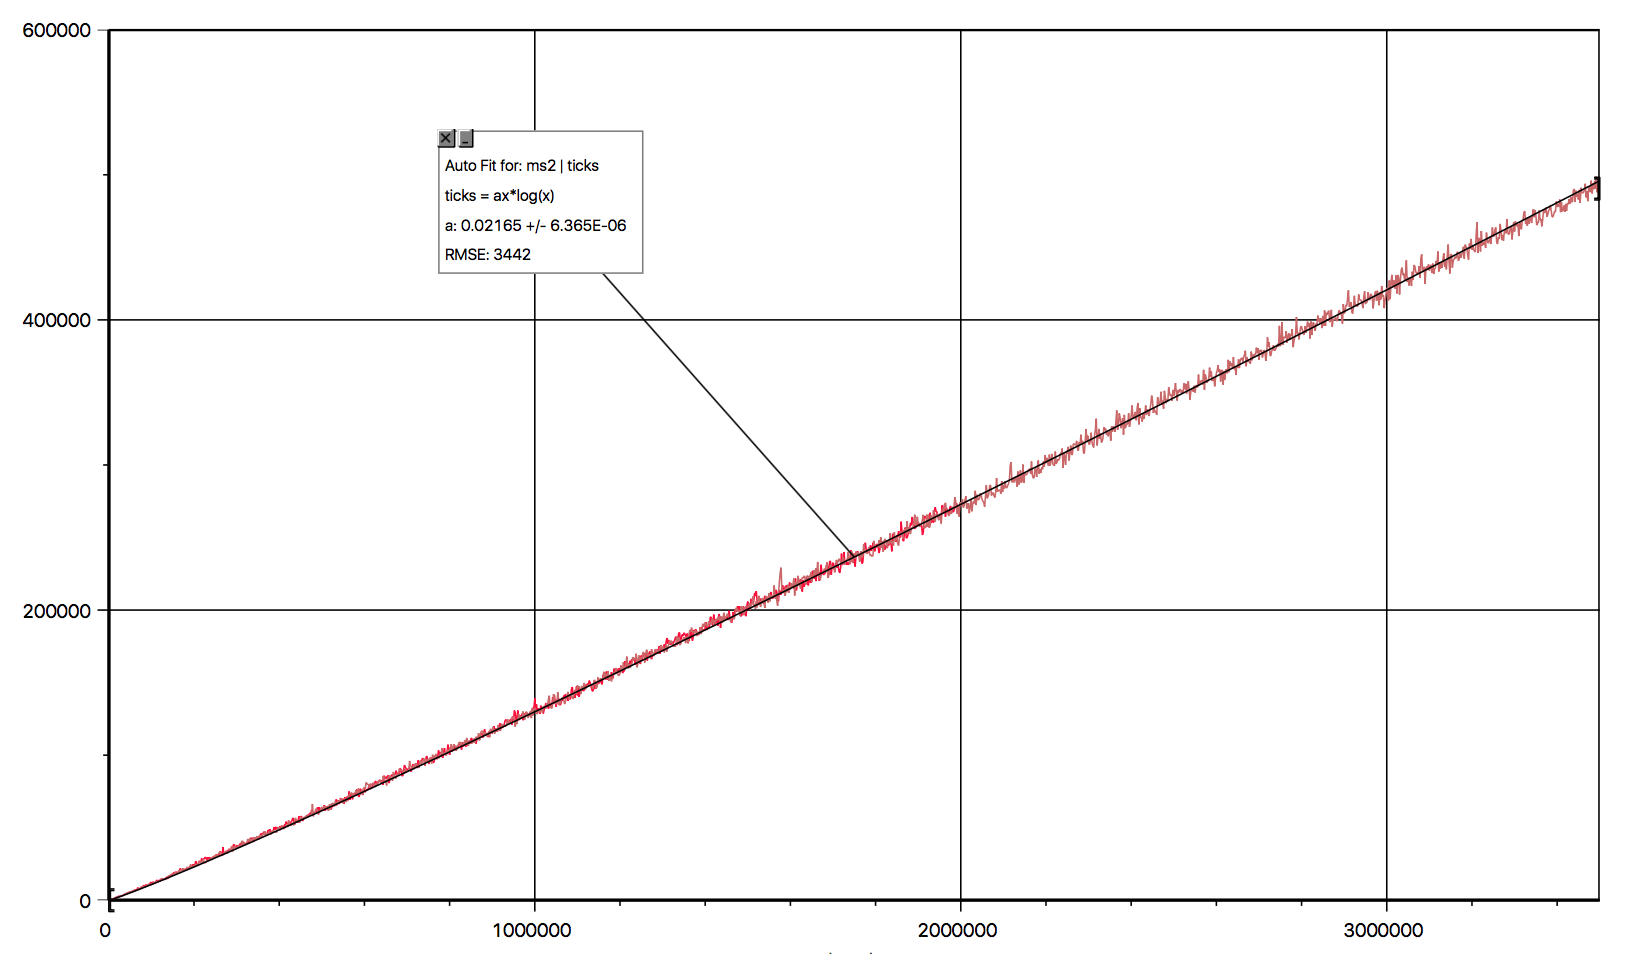
\includegraphics[width=0.3\textwidth]{ms-best.png}\label{fig:f1}}
  \hfill
   \subfloat[average-case]{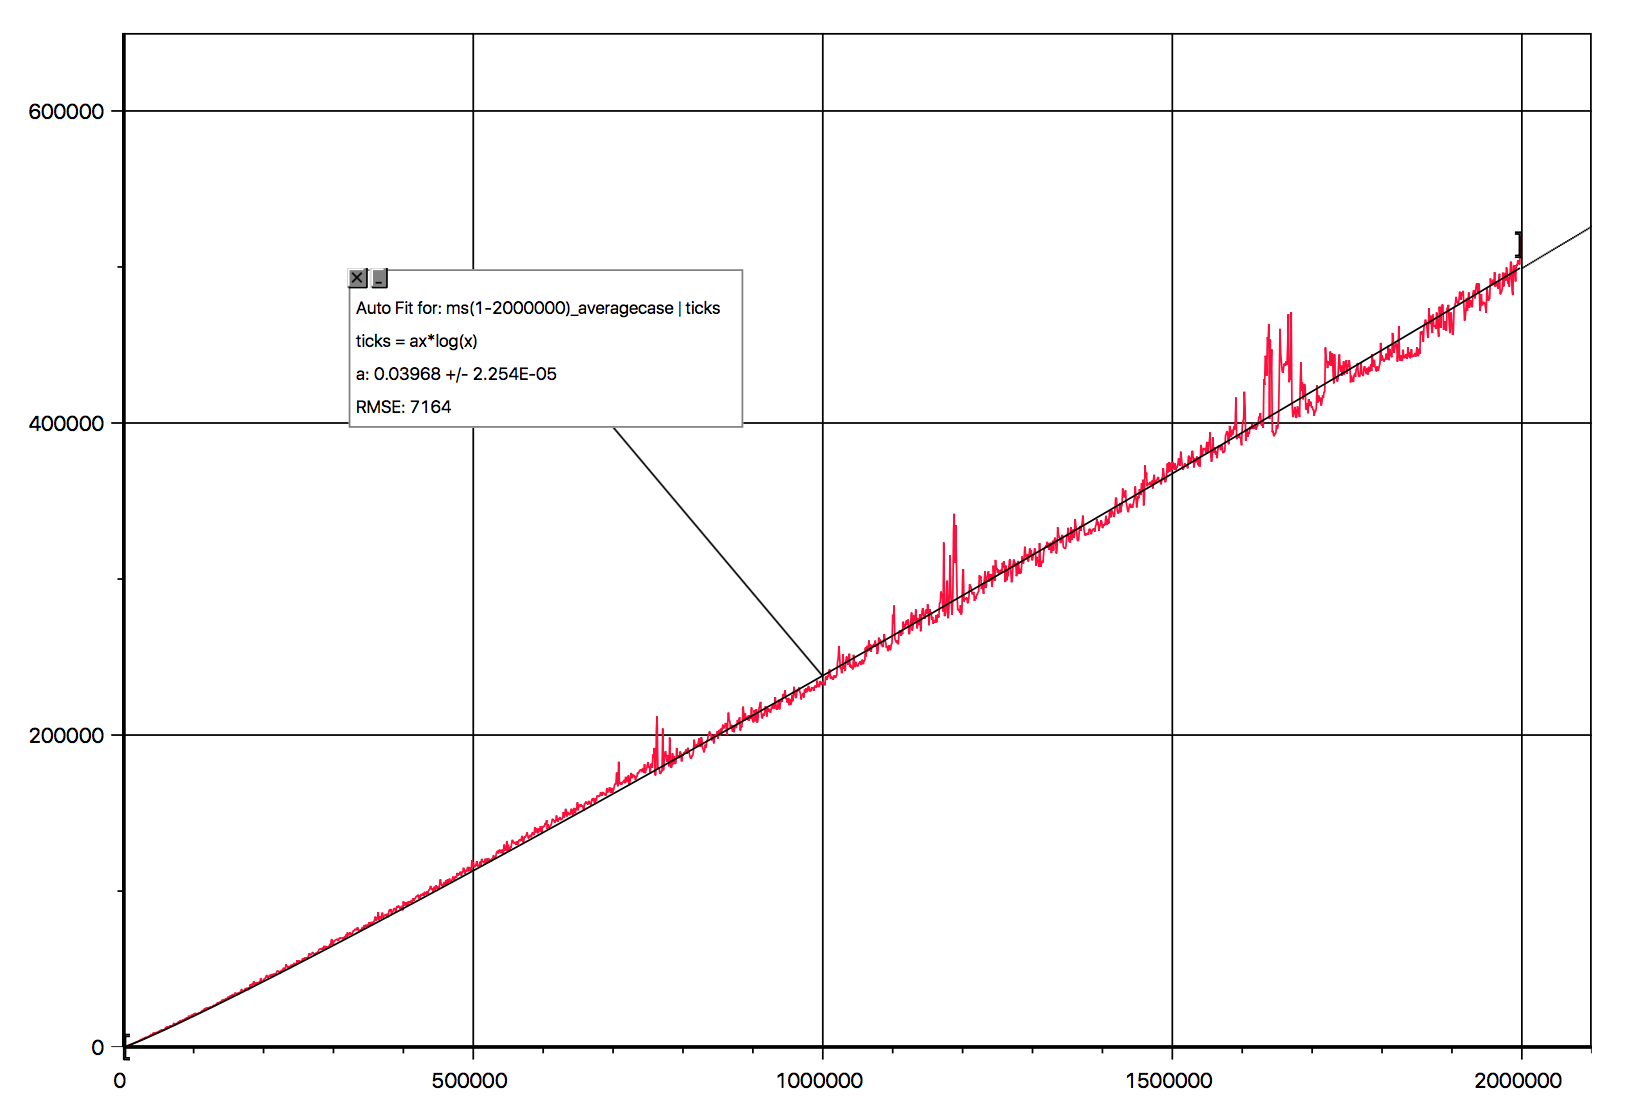
\includegraphics[width=0.3\textwidth]{ms-average.png}\label{fig:f1}}
  \hfill
  \subfloat[worst-case]{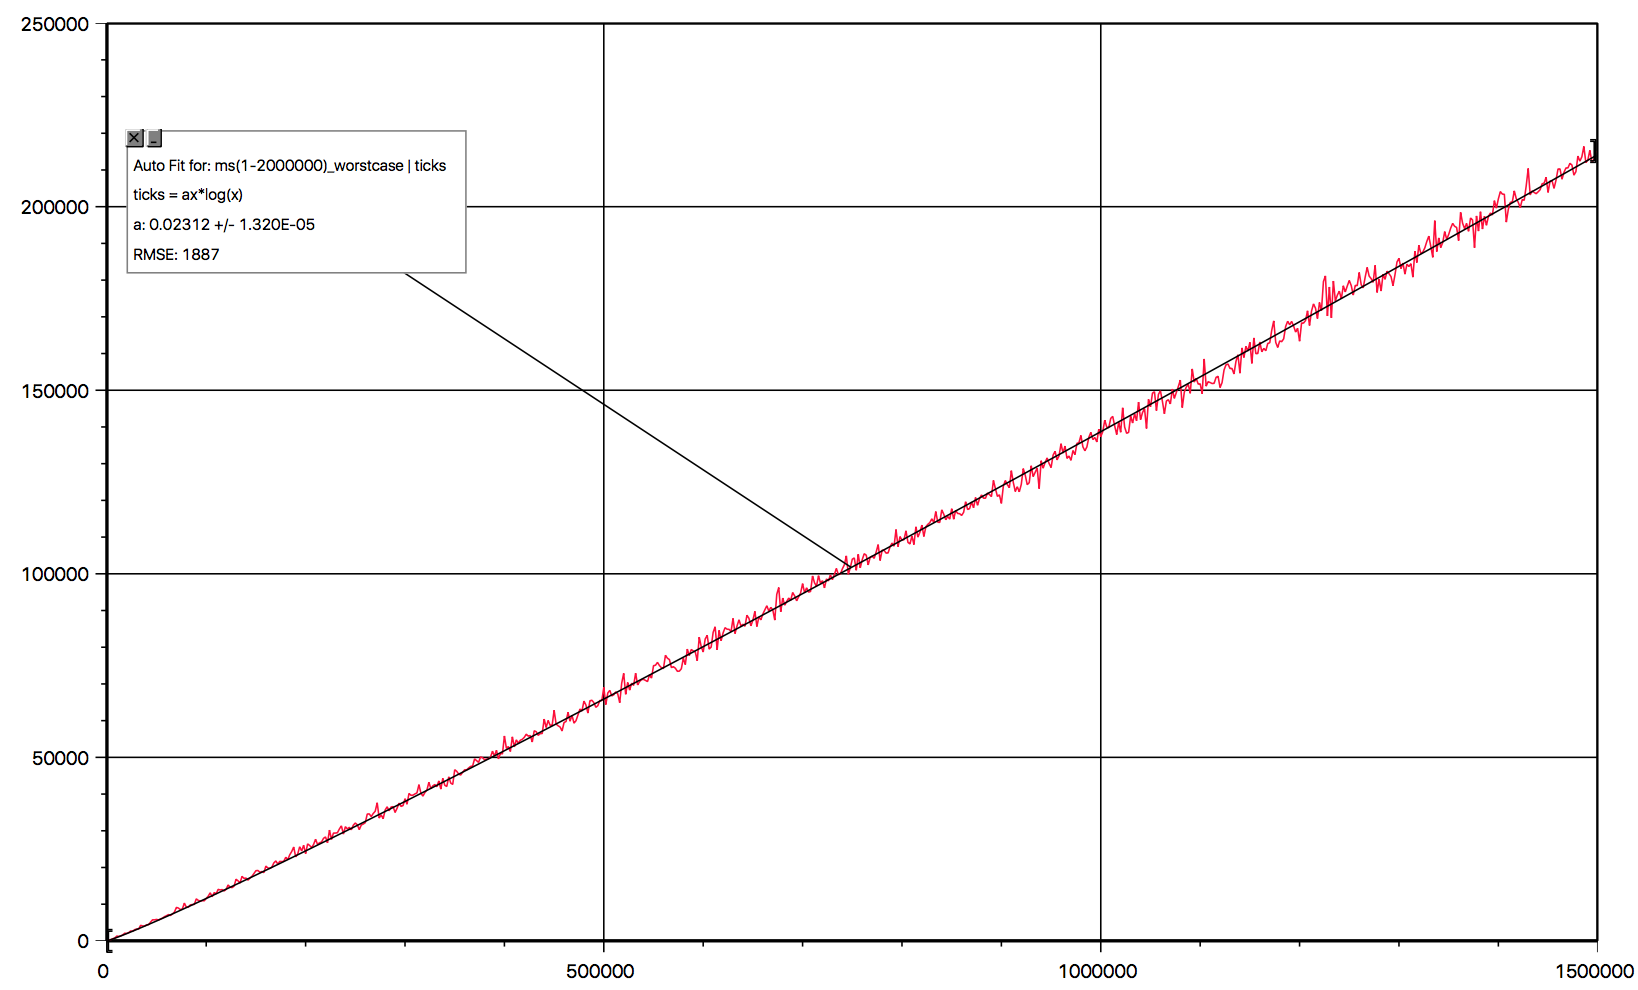
\includegraphics[width=0.3\textwidth]{ms-worst.png}\label{fig:f2}}
  \caption{Mergesort}
\end{figure}

Figures \emph{2.a}, \emph{2.b}, and \emph{2.c} above show mergesort's runtime behavior in the best, average and worst-case respectively. Contrary to many sorting algorithms, mergesorts best-case actually occurs when given a sorted array of unique elements, where its worst case occurs when the relational ordering of the array induces $n-1$ comparisons for each level. As such, series of sorted arrays were used to test the best-case behavior, randomized arrays were used to test the average case behavior, and a special algorithm was used for constructing arrays to induce the worst-case behavior.
Using (5), an RMSE comparison between attempted linear, logarithmic, and quadratic fit-attempts show that in the average-case, $n\log{}(n)$ is approximately a 16.4\% closer fit than with $a \cdot n$ and approximately a 21.5\% closer fit than with $a \cdot n^2$. Comparable differences are found in an RMSE analysis on the best and worst case - leading to empirical support for the asymptotic promise of $\Theta(n\log{}(n))$ membership in \emph{all} cases.
Although the gathered evidence supports a complexity class membership of $n \log{}(n)$ for each case, a second implication from the asymptotic promises may be investigated. If in the worst-case mergesort must make $n-1$ comparisons and in the best-case only $\frac{1}{2}n-1$ comparisons must be made then we would expect to see a constant factor of the best-case approximately half that of the worst-case (twice as fast). 

However an application of a modified (5) for \emph{expected} values to $2 \cdot a_{worst}, a_{best}$, the fit-constants generated by LoggerPro, yields an unacceptable 46.61\% error from our anticipated value. Looking closer, we see that the fit-constant, $a_{best}$ differs only marginally from $a_{worst}$. This unsettling result may be due to a lack of proportionality between our basic operation (comparison) and the total run time of mergesort for that length; stack set up, swaps, etc. may be contributing to dilute the fit-constants relationship with the total number of comparisons.

\subsection*{Quicksort Results}
\begin{figure}[h]
  \centering
  \subfloat[average case]{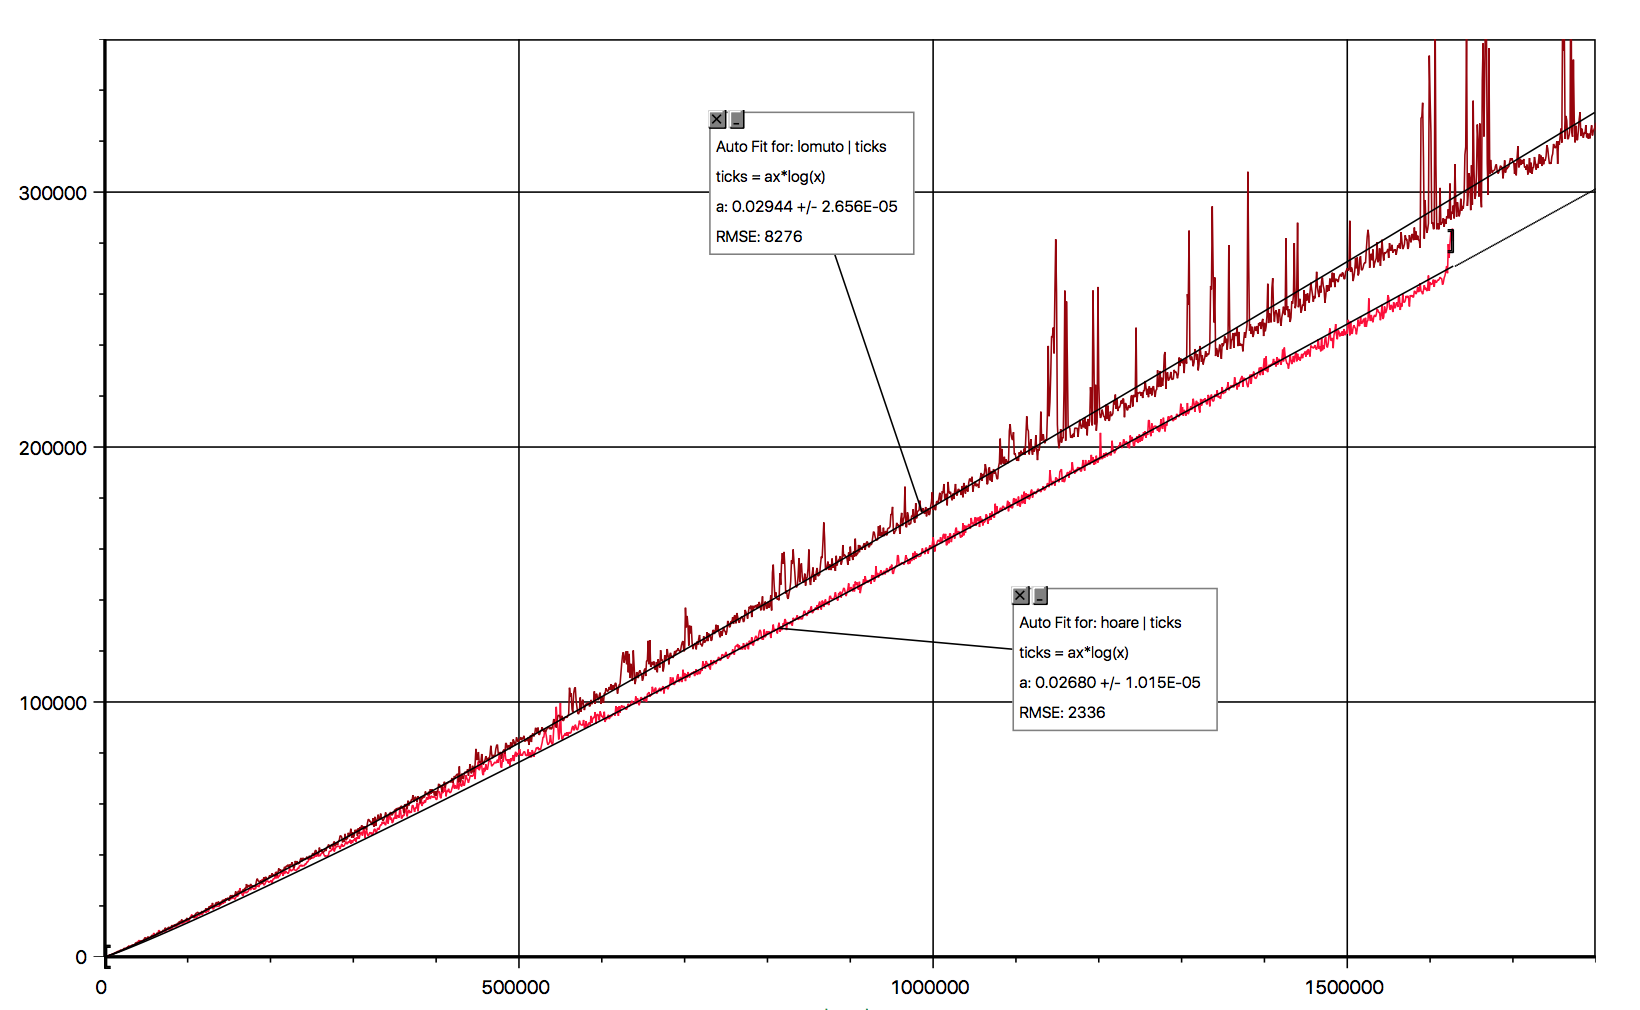
\includegraphics[width=0.5\textwidth]{qs-average.png}\label{fig:f1}}
  \hfill
  \subfloat[worst-case]{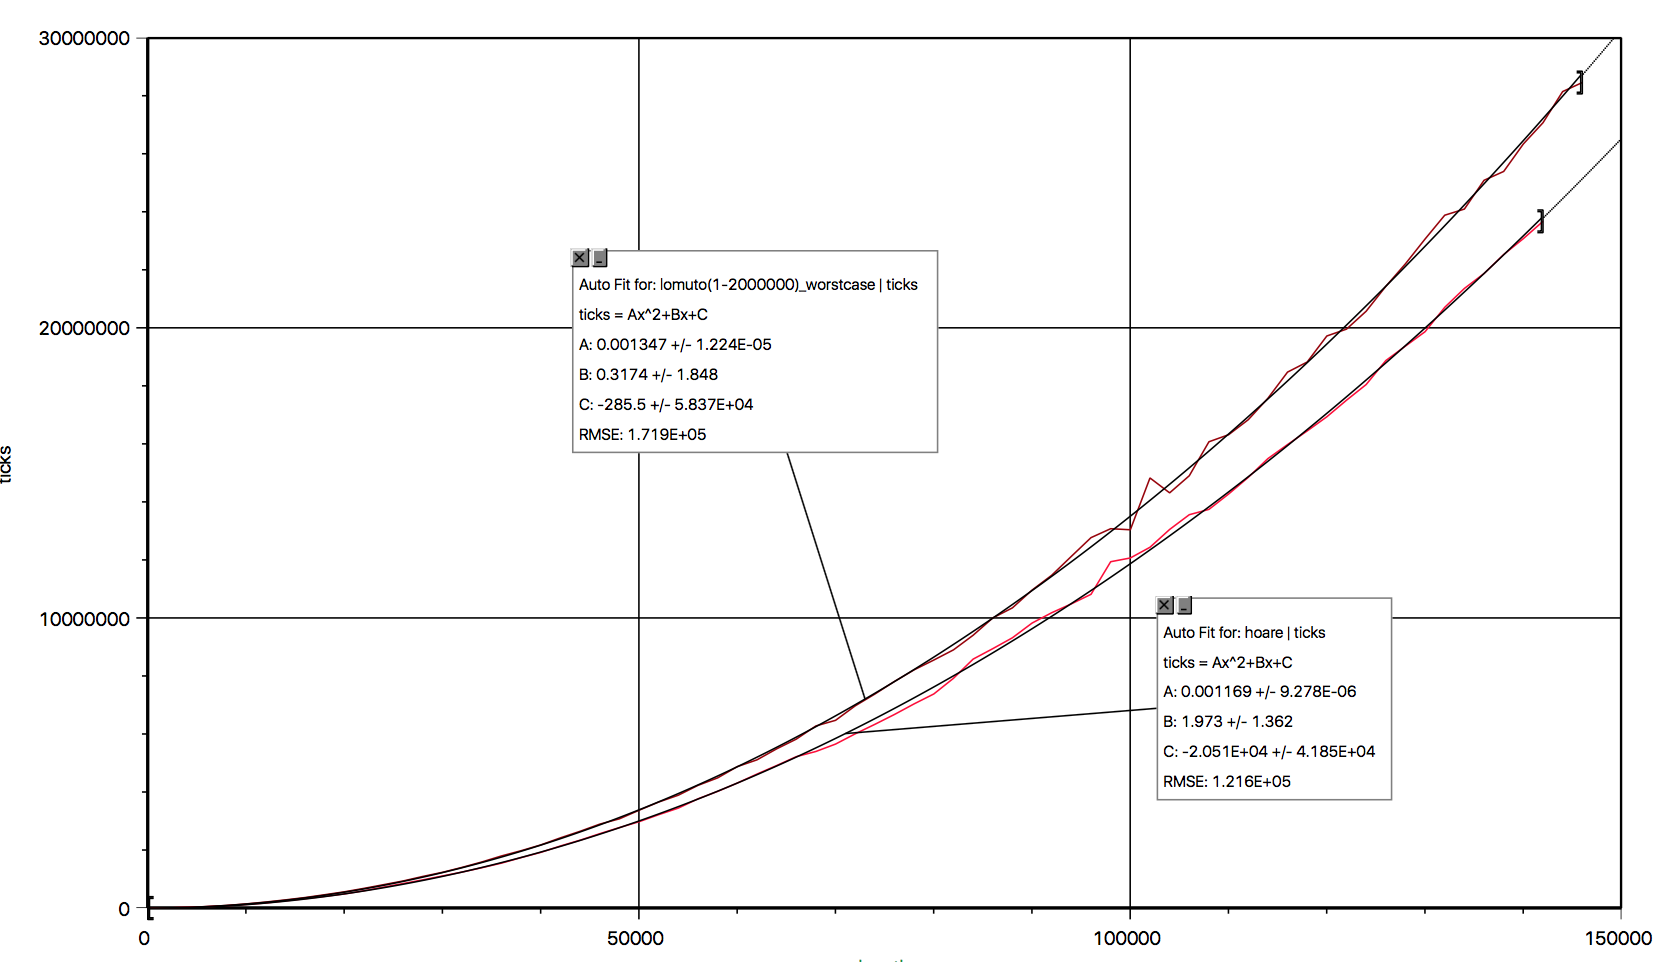
\includegraphics[width=0.5\textwidth]{qs-worst.png}\label{fig:f2}}
  \caption{Quicksort}
\end{figure}

In both \emph{Figure 1.a} and \emph{Figure 1.b} the dark-red tend line shows the runtime of quicksorts implementation using Lomuto's partitioning scheme, while the light red line is quicksorts implementation using Hoare (no best-case was tested here). An RMSE analysis from all three curve fit attempts show that regardless of the partitioning scheme employed quicksort in the average case belongs to the complexity class $\Theta (n \log{}(n))$ and in the worst case belongs to $\Theta(n^2)$. Additionally, a ratio of the two fit-constants in both cases shows that Hoare holds a slight advantage with an average-case runtime speed 8.97\%, and a worst-case runtime speed 13.21\% faster than Lomuto. However, what truly solidifies Hoare as the partitioning victor is the stability of its runtime trend line in the average case where Lomuto's implementation possesses a clear volatility. It might then be asserted, since by probability some arrays in the average case will be more sorted than others, that this volatility supports the assertion that Lomuto's partitioning scheme is more susceptible to run-times in the worst case. Some skepticism may be warranted here as the quantifiable range of fluctuation is severe and may be ascribed to inconsistencies stemming from the use of clock() - to rule this out further tests assessing runtime versus entropy for each partitioning scheme must be conducted (this is outside the scope of the current analysis).


\section*{Retrospective} % Personal review
In hindsight many things could have been improved upon throughout this project. Primarily, attempts to use the University server as a testing ground proved unsuccessful. Even with 16+ CPUs, the use of tmux and more memory than was necessary for this project, all data produced by the programs in this environment showed a wide range of reliability when analyzing the graphs. I suspect this is due to an average of 30 or more people logged in at any given time. This hiccup was circumvented by running each test locally while minimizing parallel processes. Testing procedures also could have been improved dramatically given a utility to measure \emph{user time}; unfortunately, a utility like this was not found. Additional hinderances ranged from anomalous runtimes depending on the parity of the arrays length, to the realization through analyzing data that averaging set sizes larger than three generally produced the same value. Using smaller set sizes for averaging would have allowed for faster testing and larger arrays, which in turn would have graphically illustrated the $n \cdot log{}n$ tend behavior (it is hard to differentiate between logarithmic and linear slopes in lower ranges).

In spite of the many difficulties and minute frustrations along the way, the project proved tremendously successful in demonstrating the accuracy of each algorithms asymptotic promise. Broad implications outside the scope of the analysis found in the results section center around which of these two preeminent sorting algorithms is superior. The conclusion here is, it depends. As it may have been predicted from the beginning, the choice between the two depends heavily on the value of space over time and on the range of problem instances which the algorithm must solve. If a space efficiency of $\Theta(n)$ is non negotiable and the input is guaranteed to be relatively random, then quicksort is clearly the way to go (for relatively ordered arrays, insertion sort should be considered instead). However, if space is not an issue then mergesort is clearly superior given it's performance regardless of input. 

As a personal aside, it was a very engaging and fruitful effort. 

\end{document}